Se desarrollan 4 modelos: un modelo ARIMA como base de comparación, un modelo LSTM, un modelo CNN y un híbrido LSTM-CNN.

\section{ARIMA}
Los modelos ARIMA (Autoregressive Integrated Moving Average) son una tipo de modelos estadísticos utilizados históricamente para el análisis y la predicción de series temporales
univariable. 

Utilizamos como base de comparación los resultados de un ARIMA para cada serie temporal: cada variable en cada ubicación y cada fuente de datos.

Para emplear un modelo ARIMA, es necesario ajustar cada uno de sus parámetros, que son:
\begin{itemize}
    \item $p$: el número de términos autorregresivos (AR).
    \item $d$: el número de diferencias necesarias para hacer la serie estacionaria (I).
    \item $q$: el número de términos de media móvil (MA).
\end{itemize}

\subsection{Calibración de térmios autorregresivos}
Para determinar el número de términos autorregresivos, se utiliza la función \texttt{plot\_pacf} de la librería \texttt{statsmodels}, 
que permite visualizar la función de autocorrelación parcial (PACF) de la serie temporal. Observamos ejemplos de los resultados en las figuras \ref{arima_pacf_hum}, \ref{arima_pacf_pres}. 

\begin{figure}[H]
    \centering
    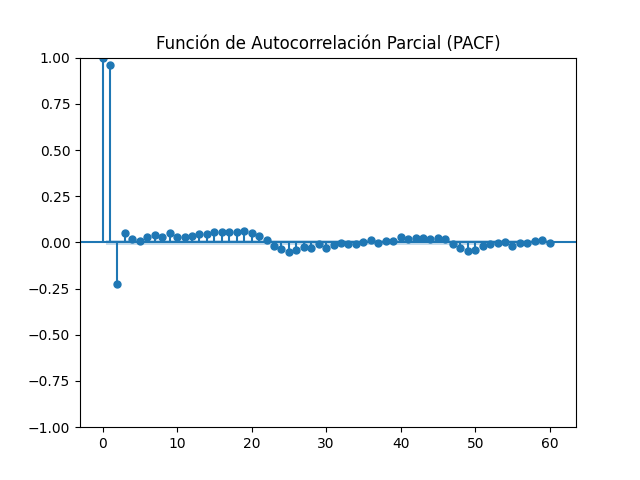
\includegraphics[width=0.5\textwidth]{images/arima_pacf_hum.png}
    \caption{Gráfico de PACF para la serie de humedad relativa en La Laguna de Grafcan}
    \label{arima_pacf_hum}
\end{figure}

\begin{figure}[H]
    \centering
    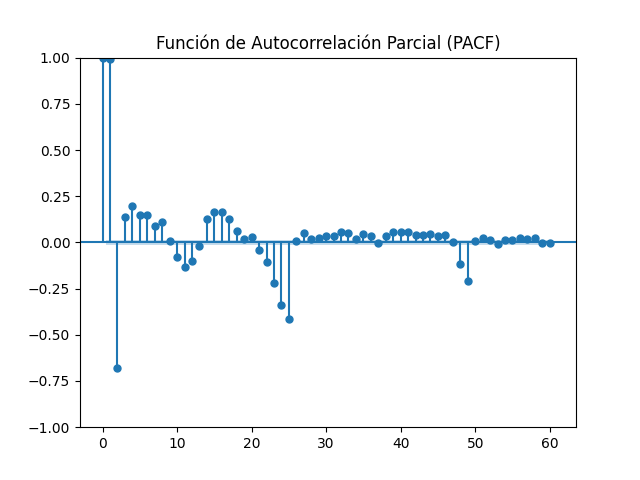
\includegraphics[width=0.5\textwidth]{images/arima_pacf_pres.png}
    \caption{Gráfico de PACF para la serie de presión atmosférica en La Laguna de Grafcan}
    \label{arima_pacf_pres}
\end{figure}


Analíticamente, se emplea el algoritmo descrito en \ref{pacf_ar_order}. Se determina $p$ = 4 para las series de temperatura del aire y humedad relativa, mientras 
que se obtiene $p$ = 8 en el caso de la presión atmosférica.

\begin{figure}[H]
    {\small
    \hrule \
    {\bf\small Pseudocódigo Selección de Orden AR vía PACF}
    \hrule
    \begin{center}
    \begin{tabbing}
    \ 1: {\bf Fun}\={\bf ción} seleccionar\_orden\_AR($serie$, $max\_lags$): \\
    \ 2: \> \# 1. Calcular la PACF hasta $max\_lags$ retardos \\
    \ 3: \> $pacf\_valores$ = PACF($serie$, $nlags$=$max\_lags$) \\
    \ 4: \> \# 2. Definir intervalo de confianza al 95\% \\
    \ 5: \> $intervalo\_confianza$ = 1.96 / raiz\_cuadrada(longitud($serie$)) \\
    \ 6: \> \# 3. Buscar el primer retardo no significativo \\
    \ 7: \> {\bf Para} \= $lag$ {\bf en} 1 \dots $max\_lags$: \\
    \ 8: \> \> {\bf Si} \= valor\_absoluto($pacf\_valores[lag]$) $<$ $intervalo\_confianza$: \\
    \ 9: \> \> \> imprimir("El mejor orden AR sugerido por la PACF es:", $lag-1$) \\
    \ 10: \> \> \> {\bf Retornar} $lag-1$ \\
    \ 11: \> \# 4. Si todos los retardos son significativos \\
    \ 12: \> imprimir("Todos los retardos hasta", $max\_lags$, "son significativos.) \\
    \ 13: \> {\bf Retornar} $max\_lags$ \\
    \end{tabbing}
    \end{center}
    \hrule
    }
    \caption{Pseudocódigo para Selección de Orden AR usando PACF}
    \label{pacf_ar_order}
\end{figure}

\subsection{Estudio de la estacionariedad}
Se emplea la prueba de Dickey-Fuller aumentada (ADF) para determinar la estacionariedad de las series temporales.
La prueba ADF es una prueba estadística que evalúa la presencia de una raíz unitaria en una serie temporal, lo que indica si la serie es estacionaria o no.
La hipótesis nula de la prueba ADF establece que la serie temporal tiene una raíz unitaria, lo que implica que no es estacionaria.
Si el valor p de la prueba es menor que un nivel de significancia predefinido (por ejemplo, 0.05), se rechaza la hipótesis nula y se concluye que la serie es estacionaria.

Empleamos como significancia un nivel de 0.05, y se obserca que todas las series temporales son estacionarias, por lo que no es necesario aplicar diferencias, 
es decir, $d$ = 0.

\subsection{Determinación del orden de la media móvil}
Para calcular el número de términos de media móvil, se utiliza la función de Autocorrelación \texttt{ACF} de la librería \texttt{statsmodels}. Dicha función 
retorna los coeficientes de autocorrelación para diferentes retardos.

Analíticamente, se emplea el algoritmo descrito en \ref{acf_ma_order}, cuya idea principal consiste en comprobar para cada retardo si el 
coeficiente de autocorrelación es significativo, finalizando cuando se encuentra el primer retardo no significativo. 

Se calcula el intervalo de confianza como 1.96 por la raíz cuadrada de la longitud de la serie temporal, ya que la distribución de
la autocorrelación estimada en cualquier lag se aproxima a una distribución normal con media 0 y desviación estándar $\frac{1}{\sqrt{n}}$,
donde $n$ es el número de observaciones. De esta forma se obtiene un intervalo de confianza al 95\% para la autocorrelación. No obstante, se establece 
un límite inferior de 0.05 para evitar que el nivel de significancia sea demasiado bajo y se detecte el ruido como una señal significativa.
\begin{figure}[H]
    {\small
    \hrule \
    {\bf\small Pseudocódigo Selección de Orden MA vía ACF}
    \hrule
    \begin{center}
    \begin{tabbing}
    \ 1: {\bf Fun}\={\bf ción} seleccionar\_orden\_MA($serie$, $max\_lags$, $min\_confidence$): \\
    \ 2: \> \# 1. Calcular la ACF hasta $max\_lags$ retardos \\
    \ 3: \> $acf\_valores$ = ACF($serie$, $nlags$=$max\_lags$) \\
    \ 4: \> \# 2. Definir intervalo de confianza al 95\% \\
    \ 5: \> $intervalo\_confianza$ = max(1.96 / raiz\_cuadrada(longitud($serie$)), $min\_confidence$) \\
    \ 6: \> \# 3. Buscar el primer retardo no significativo \\
    \ 7: \> {\bf Para} \= $lag$ {\bf en} 1 \dots $max\_lags$: \\
    \ 8: \> \> {\bf Si} \= valor\_absoluto($acf\_valores[lag]$) $<$ $intervalo\_confianza$: \\
    \ 9: \> \> \> imprimir("El mejor orden MA sugerido por la ACF es:", $lag-1$)\\
    \ 10: \> \> {\bf Retornar} $lag-1$\\
    \ 11: \> {\bf Retornar} $max\_lags$\\
    \end{tabbing}
    \end{center}
    }
    \hrule
    \caption{Pseudocódigo para Selección de Orden MA usando ACF}
    \label{acf_ma_order}
\end{figure}

El algoritmo descrito retorna el máximo número de retardos para valores elevados de lags, por lo que se analiza el gráfico de la ACF y se observa que
no existe un punto de corte claro, sino que existe un descenso suave y progresivo para todas las variables \ref{acf_arima_temp} \ref{acf_arima_pres}. Por lo tanto, se fija $q$ = 0.

\begin{figure}[H]
    \centering
    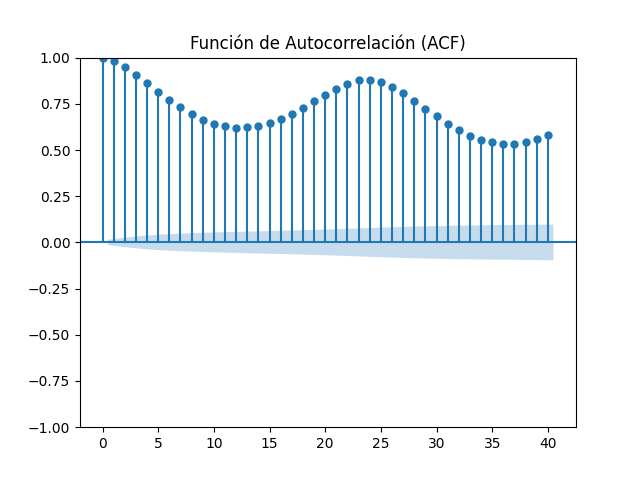
\includegraphics[width=0.5\textwidth]{images/arima_acf_temp.png}
    \caption{Gráfico de ACF para la serie de temperatura del aire en La Laguna de Grafcan}
    \label{acf_arima_temp}
\end{figure}

\begin{figure}[H]
    \centering
    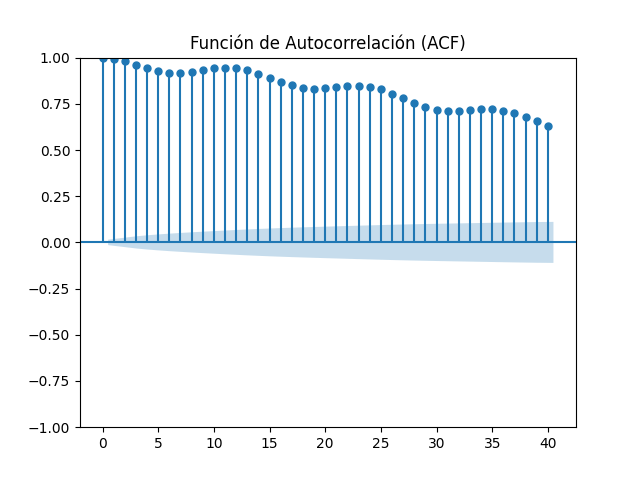
\includegraphics[width=0.5\textwidth]{images/arima_acf_pres.png}
    \caption{Gráfico de ACF para la serie de presión atmosférica en La Laguna de Grafcan}
    \label{acf_arima_pres}
\end{figure}

\section{Modelos de aprendizaje profundo}
Existen diferentes frameworks para el desarrollo de modelos de aprendizaje profundo, destacando TensorFlow, PyTorch o JAX/Flax como los más extendidos.
Después de evaluar alternativas, se opta por TensorFlow debido a su amplia comunidad de usuarios y su extensa documentación, así comopor su integración con Keras, 
una biblioteca de alto nivel que facilita la creación de modelos de aprendizaje profundo.

\subsection{LSTM}

\subsection{CNN}

\subsection{LSTM-CNN}


\section{Comparativa inicial}
Realizar una comparativa justa entre los modelos ARIMA y los modelos de aprendizaje profundo es imposible, debido a que tienen naturalezas distintas.
Los 

\section{Estudios empíricos}

\subsection{Número de estaciones}
Se estudia el impacto del número de estaciones en la precisión de los modelos. Se entrena un modelo LSTM con diferente número de estaciones. Los resultados se muestran en la tabla XXX.
Para evaluarlo, se mide el desempeño frente a las estaciones de test. Observamos que el rendimiento mejora a medida que se añaden más estaciones.

\subsection{Tamaño de la ventana}

\subsection{Uso de ruido}

\section{Resultados}
\subsection{Temperatura del aire}
\subsection{Humedad relativa}
\subsection{Presión atmosférica}

